\documentclass[../../main.tex]{subfiles}

\begin{document}

\subsection{Planlægning}
Planlægningsafsnittet beskriver planlægningen af elaborationsfasen. Dette gøres ved at beskrive overordnede artefakter, som produkt backlog, sprints, roller, ceremonier, Scrumbuts, og de enkelte iterationer.

\paragraph{Tidslinje med faser og milepæle}\mbox{}\\
På figur \ref{fig:tidslinje} vises den overordnede tidslinje for projektforløbet. Her indgår deadlines, og de forskellige faser under projektforløbet. Denne tidslinje har været med til at skabe et overblik over hele projektforløbet. Milepæle er modelleret med grønne og blå farver.

\begin{figure}[H]
  \centering
  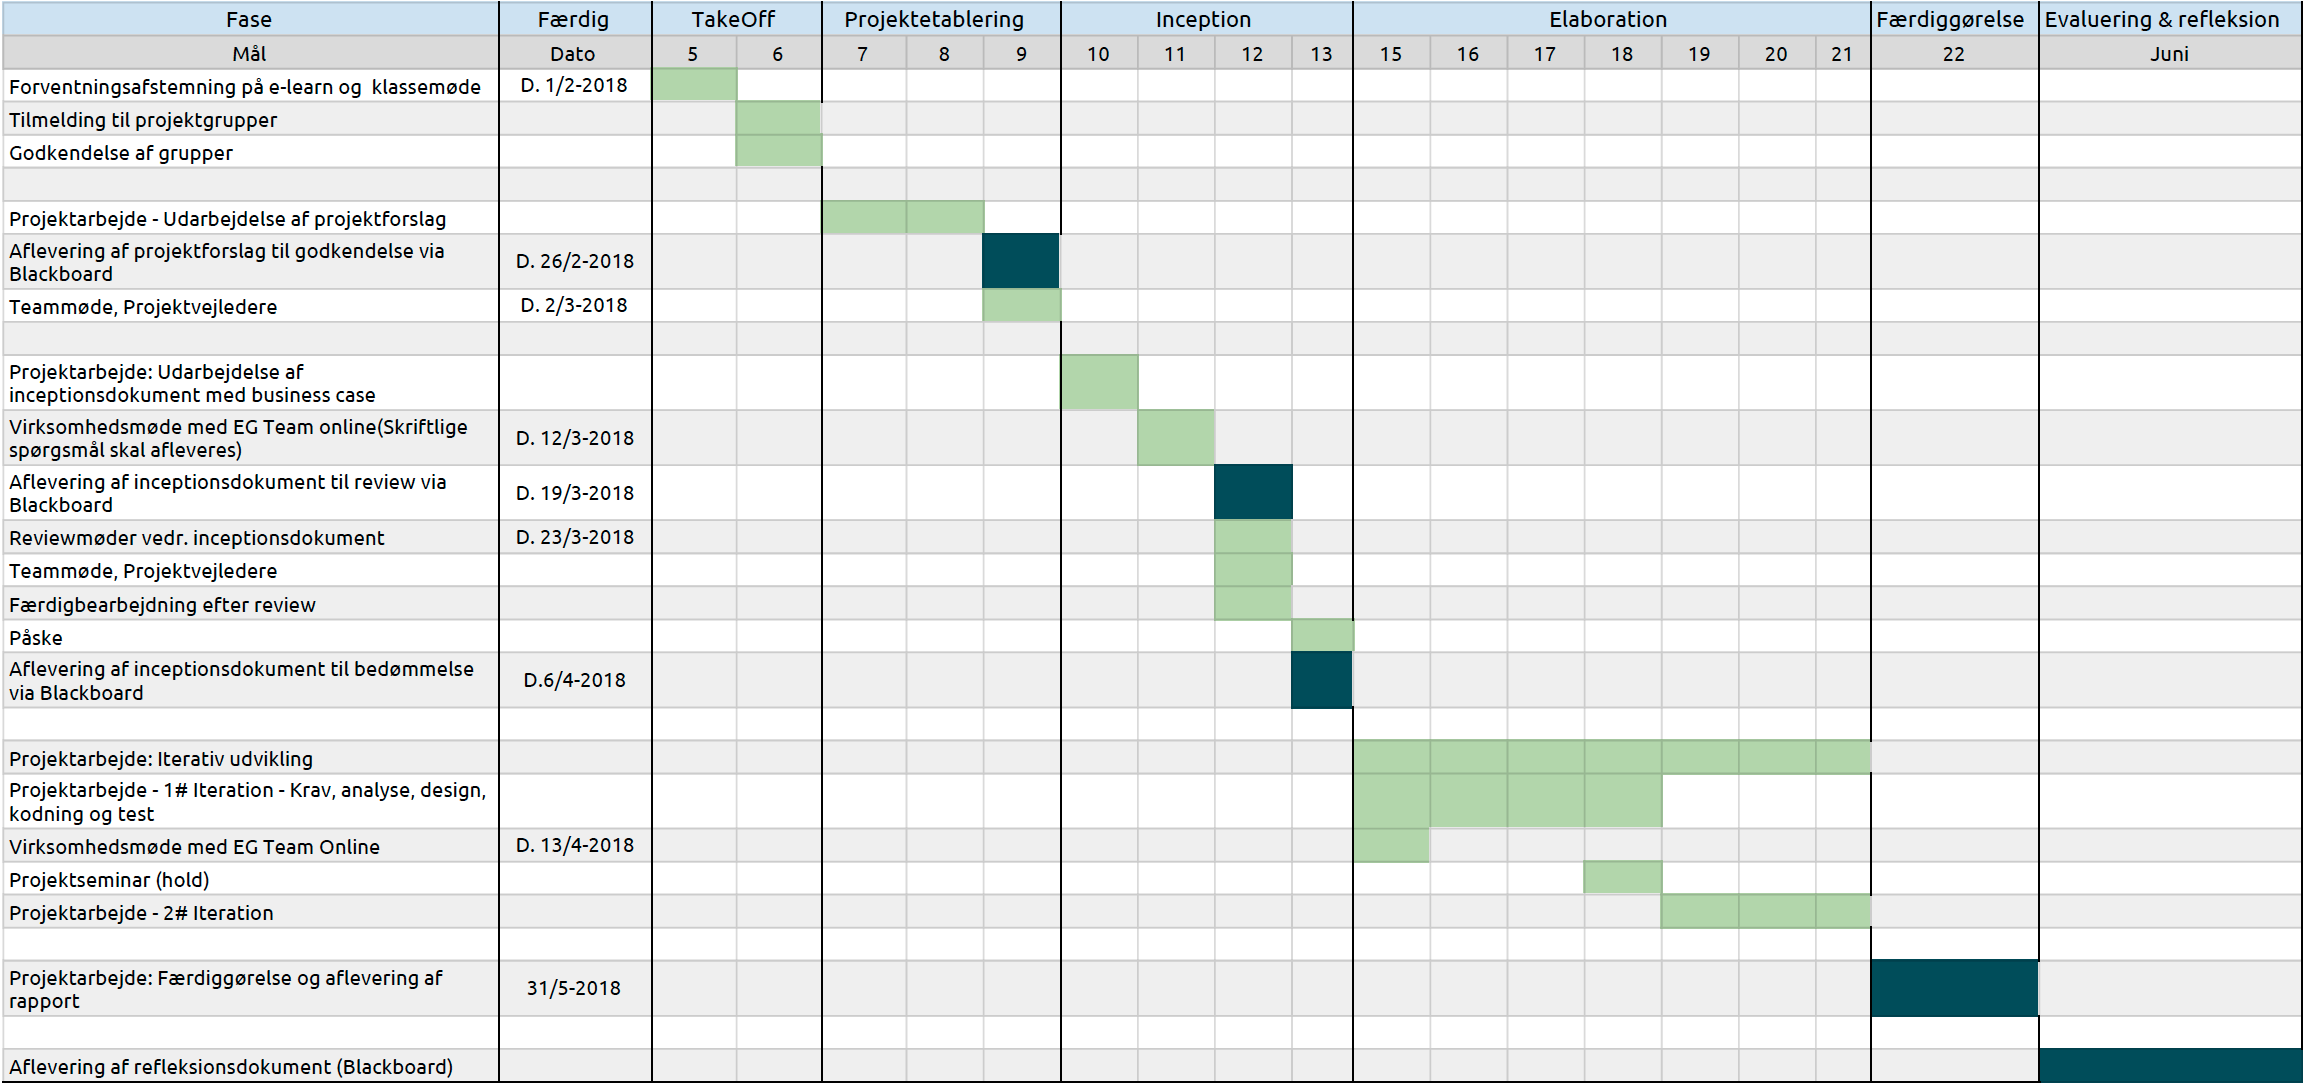
\includegraphics[scale=.4]{figurer/milep_l.png}
  \caption{Gant diagram med milepæle og ugernumre}
  \label{fig:tidslinje}
\end{figure}

\paragraph{Sprints}\mbox{}\\
Vi valgte at sprints skulle have en varighed på to uger. Vi mente at to uger passede godt i forhold til vores arbejdsform, da det vil give os en hurtig iterations cyklus, og derved gøre, at teamet er omstillingsparate i forhold til ændringer i projektforløbet, samt oftere udfører retrospektiver, hvilket forbedrer gruppens samarbejde. Ulemperne ved et t0 ugers retrospektiv kunne dog være, at det bliver svært at færdiggøre Sprint Backlogs, og der skal oftere planlægges og tilrettelægges nye sprints, hvilket der også bruges tid på. Yderligere kan en kortere iterationscyklus føre til for kortsigtet planlægning, hvor teamet vænner sig til at kunne foretage ændringer inden for 14 dages tidsintervaller. Dette kan skade tidshorisonten på gennemførslen af projektet, da der tænkes for lidt på den langsigtede planlægning. 
 

For at skabe gennemsigtighed i forhold til hvilke brugsmønstre der er påbegyndt arbejde på, og hvilken fase de er i, benytter teamet GitHub's Kanban board. Projektets Kanban board kan ses under under: \cite{github}. 
På denne måde sikrer gruppen, at der bliver taget hånd om alle brugsmønstre, der er planlagt i et sprint backloggen, og der kan hurtigt skabes et overblik over hvad der mangler. 

I sammenhæng med at teamets Kanban board vedligeholdes, så er der også et burndown diagram over hver sprint iteration. Således er der mulighed for at opdage eventuelle problemer i forhold til hvordan sprintet bliver eksekveret, og om der er nogle brugsmønstre der kan udskydes, hvis teamet er i en presset situation eller holder fokus et forkert sted.
\begin{figure}[H]
  \centering
  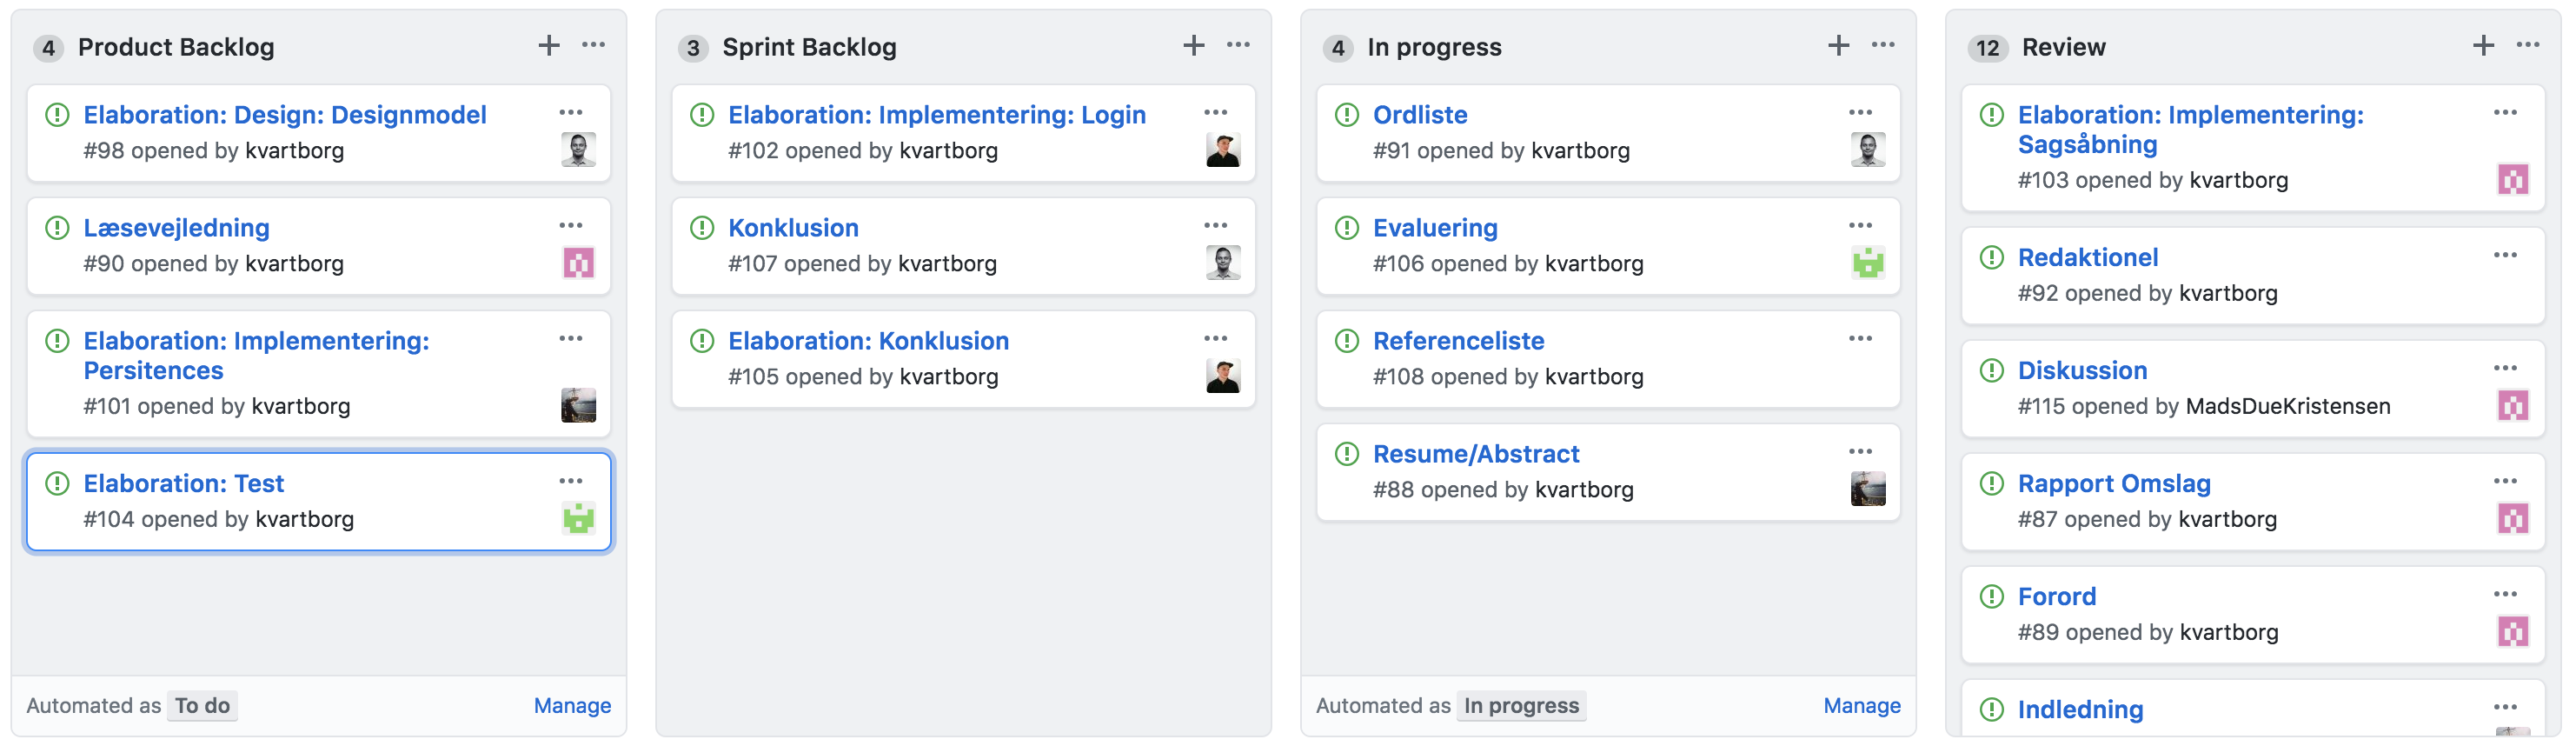
\includegraphics[scale=.29]{figurer/kanban.png}
  \label{fig:github_board}
  \caption{Teamets GitHub Board, kan ses i fuld størrelse i bilag \ref{fig:github_board_stor}}
\end{figure}


\paragraph{Roller}  \mbox{}\\
Teamet har besluttet at have en Scrum master og en product owner. Da projeket ikke har en reel kunde tilknyttet, er product owneren et gruppemedlem. 
Rollerne som Scrum master og product owner holdes af de samme medlemmer af teamet igennem hele projektet. Alle gruppemedlemmer, også de to som er scrum master og product owner, er en del af projektets "Development Team".

\paragraph{Ceremonier} \label{Ceremonier} \mbox{}\\
Gruppen har valgt at gøre følgende med ceremonierne:

\begin{itemize}
\item Sprint planning: Dette holdes i starten af hver sprint. Under dette møde planlægges den kommende sprint ved at der udvælges opgaver fra product backloggen og tilføjet til sprint backloggen. Her laves også tidsestimater til hver opgave. Disse laves med både udførelse, dokumentation og review af arbejdet for øje.
\item Daily Scrum: Dette holdes hver gang gruppen mødes. Under mødet fortæller hver gruppe medlem hvad de har lavet siden sidst, om de har nogle problemer, og hvad de planlægger at arbejde på. Efter mødet vil burndown diagrammet blive opdateret.
\item Sprint review: Dette udføres ikke, da der ikke er nogen kunde at lave review med.
\item Sprint retrospektive: Dette holdes efter hver sprint. Under dette møde diskuteres det hvad der gik godt og hvad der gik mindre godt under den afsluttede sprint, så næste sprint kan blive bedre. Et retrospective har en maksimal længde på 30 minutter, så det bliver kort og præcist.
\end{itemize}

\paragraph{Produkt Backlog}\mbox{}\\
I tabel \ref{tab:produkt_backlog} ses produkt backloggen for projektet. Elementernes tidsestimat er angivet i timer. Der er ikke en product backlog for hele Sensum Udred, men for hvad der vil blive arbejdet med inden for vores afgrænsning af projektet. 


Hver opgave i projekts produkt backlog er estimeret udfra følgende kriterier, som gruppen ser nødvendige ved analyse, implementering og test af et brugsmønster: 
\begin{itemize}
	\item Dokumentation i form af diagrammer og beskrivende tekst i rapporten.
    \item Implementering af brugsmønster i kodebasen.
    \item Test af implementeret løsning.
    \item Review af dokumentation.
    \item Review af implementering.
\end{itemize}
Udfra de ovenstående punkter har vi estimeret tiden for hvert brugsmønster ved, at alle team medlemmer hver især kom med et bud på hvor længe det enkelte brugmønster ville tage at færdiggøre, med alle ovenstående faktorer medregnet. Ud fra disse blev tidsestimaterne diskuteret og fastlagt.\\ 
Normalvis vil der kun være user-stories/brugsmønstre i product backloggen, men i og med at den er blevet benyttet til at adminstrere hele projektet, inklusiv elementer som rapportskrivning, er det blevet vurderet nødvendigt at have elementer der falder uden for brugsmønstrene i backloggen.   

\begin{center}
   \small
   \begin{longtable}{| l | c |}
    \hline
    \textbf{Opgaver}												 & \textbf{Estimat (timer)} \\ \hline
    Opsætning af tre lags arkitektur							     & 4  \\ \hline
    Analysemodel													 & 24 \\ \hline
    Basisklasse opsætning ud fra analysemodel						 & 18 \\ \hline
    Detaljeret Brugsmønster											 & 10 \\ \hline
    Kundemøde EG Team Online										 & 10 \\ \hline
    Fastlæg struktur for scrum burndown								 & 6  \\ \hline
    Persistenslag							 	 					 & 16 \\ \hline
    Implementering af simpel Login									 & 12 \\ \hline
	...																 & ... \\ \hline
    \textbf{I Alt}													 & 443 \\ \hline
    \caption{Projectes produkt backlog, se bilag tabel \ref{tab:produkt_backlog_bilag} for fuld længde}
    \label{tab:produkt_backlog}
    \end{longtable}
\end{center}

\paragraph{Sprint backlog}\mbox{} \\
Sprint backloggen indeholder de udvalgte opgaver fra product backloggen i et givent sprint. For at skabe overblik over tidsforbruget på de forskellige opgaver bliver der løbende vedligeholdt et burndown diagram, dette giver et overblik over tilbageværende tid på hver opgave og på denne måde kan det ses om sprintet afvikles som forventet.

\paragraph{Scrumbuts} \label{Scrum-buts} \mbox{}\\
Scrumbuts beskriver modifikationer til den traditionelle Scrum, og hvilke valg der er taget i stedet.
I projektet bliver der brugt følgende Scrum-buts:

(Vi bruger Scrum, men)(Vi mødes ikke hver dag)(så derfor holder der kun daglige Scrum møde på de dage hvor vi mødes) 

(Vi bruger Scrum, men)(Vi har ikke mulighed for at have en repræsentant fra EG Team Online)(så derfor er et medlem af Scrum teamet product owner i dette projekt)

(Vi bruger Scrum, men)(Vi ønsker at benytte analyse og designprocesserne fra Unified Process)(så vores backlog indeholder ikke Scrums User Stories, men derimod brugsmønstre)  

(Vi bruger Scrum, men)(Vi ønsker at alle arbejdsopgaver ligger det samme sted)(så vores backlog indeholder ikke kun brugsmønstre)  


\end{document}